\documentclass[a4paper,12pt,fleqn]{article}
\usepackage[utf8]{inputenc}
%\usepackage[latin1]{inputenc}
\usepackage{amsmath,amssymb}
\usepackage[english]{babel}
\usepackage{amssymb}
\usepackage{geometry}
\geometry{a4paper, top=25mm, left=30mm, right=30mm, bottom=30mm,
	headsep=10mm, footskip=12mm}
\usepackage{pdfpages}
\usepackage{afterpage}
% \usepackage{fourier} \usepackage[scaled=0.84]{berasans} \usepackage[scaled=0.84]{beramono}
% sets the font of text and formulae to Utopia; sets the sans-serif and monospaced font to Bera
% \usepackage{mathptmx} \usepackage[scaled=0.9]{helvet} \usepackage{courier}
% sets the font of text and formulae to Times; sets the sans-serif font to Helvetica;
% sets the monospaced font to Courier

 \usepackage[charter]{mathdesign} \usepackage{berasans} \usepackage{courier}
%\usepackage{beramono}

% sets the font of text and formulae to ITC Charter; sets the sans-serif and monospaced font to Bera
% \usepackage[osf]{mathpazo} \usepackage[scaled=0.9]{helvet} \usepackage{courier}
% sets the font of text and formulae to Palatino; sets the sans-serif font to Helvetica;
% sets the monospaced font to Courier

\frenchspacing
\sloppy
\usepackage{microtype}
\usepackage[onehalfspacing]{setspace}
\usepackage{array}

%\usepackage[pdftex]{graphicx}
\usepackage{color}
\definecolor{darkblue}{rgb}{0.00,0.00,0.50}
\definecolor{darkred}{rgb}{0.80,0.00,0.00}
\definecolor{hu-blue}{RGB}{0,55,108}
\usepackage[pdftex, pdftitle={Title of Your Document},
pdfauthor={Xiaolin Qin}, pdfsubject={Seminar Paper},
bookmarks=true, bookmarksopen=true, bookmarksnumbered=true, bookmarksopenlevel=2, colorlinks=true,
pdfpagemode=UseOutlines, pdfview=Fit, pdfstartview=Fit, pdffitwindow=false, linkcolor=hu-blue,
citecolor=hu-blue, urlcolor=hu-blue, pagebackref]{hyperref}
\urlstyle{same}
\usepackage{memhfixc}

\newcommand{\rdmatrix}[1]{\left(\,\begin{matrix}#1\end{matrix}\,\right)}
\newcommand{\sqmatrix}[1]{\left[\,\begin{matrix}#1\end{matrix}\,\right]}

\newcommand{\E}{\mathrm{E}}
\newcommand{\dd}{\mathrm{d}}   % "dd" for "differential d"
\newcommand{\Var}{\mathrm{Var}}
\newcommand{\Cov}{\mathrm{Cov}}

\usepackage[authoryear, longnamesfirst]{natbib}

\usepackage{chngcntr}
\counterwithin{figure}{section}

\usepackage{listings}

\usepackage{multirow}

\usepackage{csquotes}

\usepackage{abstract}

\usepackage{xcolor}
\definecolor{mygray1}{rgb}{0.97,0.97,1}
\definecolor{mygray2}{rgb}{0.75,0.75,0.75}
\definecolor{mygray3}{rgb}{0.7,0.7,0.7}



\usepackage{titlesec}
\usepackage{hyperref}

\titleclass{\subsubsubsection}{straight}[\subsection]

\newcounter{subsubsubsection}[subsubsection]
\renewcommand\thesubsubsubsection{\thesubsubsection.\arabic{subsubsubsection}}
\renewcommand\theparagraph{\thesubsubsubsection.\arabic{paragraph}} % optional; useful if paragraphs are to be numbered

\titleformat{\subsubsubsection}
{\normalfont\normalsize\bfseries}{\thesubsubsubsection}{1em}{}
\titlespacing*{\subsubsubsection}
{0pt}{3.25ex plus 1ex minus .2ex}{1.5ex plus .2ex}

\makeatletter
\renewcommand\paragraph{\@startsection{paragraph}{5}{\z@}%
	{3.25ex \@plus1ex \@minus.2ex}%
	{-1em}%
	{\normalfont\normalsize\bfseries}}
\renewcommand\subparagraph{\@startsection{subparagraph}{6}{\parindent}%
	{3.25ex \@plus1ex \@minus .2ex}%
	{-1em}%
	{\normalfont\normalsize\bfseries}}
\def\toclevel@subsubsubsection{4}
\def\toclevel@paragraph{5}
\def\toclevel@paragraph{6}
\def\l@subsubsubsection{\@dottedtocline{4}{7em}{4em}}
\def\l@paragraph{\@dottedtocline{5}{10em}{5em}}
\def\l@subparagraph{\@dottedtocline{6}{14em}{6em}}
\makeatother

\setcounter{secnumdepth}{4}
\setcounter{tocdepth}{4}


\usepackage{graphicx}
\usepackage{grffile}

%%%%%%%%%%%%%%%%%%%%%%%%%%%%%%%%%%%%%%%%%%%%%%%%%%%

\begin{document}


\begin{titlepage}
	\thispagestyle{plain}
	\begin{figure*}[h]
		\centering
		
\includegraphics[width=0.3\linewidth]{Huberlin-logo.svg}
	\end{figure*}
\hrule
 \vspace{10pt}
\centering{{\LARGE \textbf{A Study of Various Clustering Algorithms for Sets of Mixed Data Types \\\vspace{15pt} \large Application to Data from an Online Fashion Retailor}}} \vspace{10pt}
\hrule
\vspace{50pt}
{\Large Seminar Statistical Programming Languages}\\[10pt]
{\Large Lecturer: Alla Petukhina}\\[10pt]
{\Large Ladislaus von Bortkiewicz Chair of Statistics}\\ 
{\large School of Business and Economics}\\  
{\large Humboldt-Universit\"{a}t zu Berlin \vspace{30pt}}\\
\url{https://github.com/tangyumei/SS18-SPL-Project}\\[30pt]
\begin{tabular}{lr}
	Nikolaus Grefe & 591705\\
	Artsem Nikifarau & 592847 \\
	Xiaolin Qin & 527054\\
	Yumei Tang & 528172\\
	Qong Wu & 528170\\	
\end{tabular}

\vspace{50pt}
\today
\pagenumbering{gobble}
\end{titlepage}



\newpage
\pagenumbering{roman}
\setcounter{tocdepth}{3}
\tableofcontents





\newpage
\addcontentsline{toc}{section}{List of Tables}
\listoftables


\addcontentsline{toc}{section}{List of Figures}
\listoffigures




\newpage\null\thispagestyle{empty}
\vspace{\fill}
\begin{figure}[h]
	\centering
\emph{This page is intentionally left blank}
\end{figure}
\vspace{\fill}
\newpage
\pagenumbering{arabic}
\section{Introduction}
With the explosion in e-commerce, extracting the hidden knowledge from the sales/customer databases has become a growing need for a business wanting to be successful. By identifying high-value customers, retaining them and even bring lower-value customers to a higher cluster, firms can achieve greater profitability. Classification and patterns extraction from customer data thus provides strong support for business decision making, which motivates us to use several different clustering algorithms in order to determine which one could have better performance on our datasets for clustering.

A large body of work has been done on existing clustering method for retail data. Mathew et al.(2015) discussed different clustering techniques which can be used in sales databases, through comparing their advantages, limitations as well as the strengths of their role in business decision making, it provides us a benneficial overview of existing solutions for classification and clustering techniques. Sankar and Rajagopal (2011) used data mining techniques on retail smart data, classifying existing customer cluster  methods into methodology-oriented and application-oriented approaches, and tried to identify the high-value and low-risk customers, which proves that the proposed approach in his study helps identification. Bilgic et al. (2017) analyzed a supermarket chain company by using a hierarchical clustering method, and then they applied frequent itemsets and association rules analysis to implement target marketing.

In this report, we apply different clustering techniques on one online retailing transaction data to evaluate the effectiveness of different algorithm and further achieve customer segmentation. Retail sales is an important issue in the market. Various literature has covered this area to extract information on market patterns, customer behaviour, demand and supply ect. The data we use in this report comes from an online fashion retaining transaction database, which is originally order ID oriented with user information, product information and order information. To form a better understanding of customer features, we identify customer segments by age, gender, state and loyalty, i.e. changing identification from order\_item to user\_id, and create a new variable RFM(Recency, Frequency and Monetary Value) to represent customer value. Since our data after transformed is user-information oriented, we know better about customer segmentation.

This report proceeds as follows. After we introduced the background of the topic in this chapter 1, we explain the definition of RFM and the theory of cluster techniques we use in chapter 2. The Theoretical foundation of this paper includes partitioning algorithms (including PAM and K-means algorithms), hierarchy algorithms (including agglomerative clustering and divisive clustering) and the DBSCAN algorithm. We implement different clustering techniques to our data and report the empirical study results and analysis in chapter 3. Finally, we compare different techniques and reach a conclusion.

\newpage
\section{Definition and Theory}
This theory section follows the notation and structure of Härdle et al. (2003) and Tan et al. (2013). It covers the RFM and the diverse clustering techniques, starting with partitioning and hierarchical approaches and closing with density based clustering.

\subsection{RFM}
In this report, we determine customer value by the RFM measure, an index accounting for:
\begin{itemize}
	\item Recency (R):\- How recently did the customer purchase?
	\item Frequency (F):\- How often does the customer purchase in a specific time period?
	\item Monetary (M):\- How much does the customer spend in a specific time period?
\end{itemize}

\subsection{Clustering}%2.2
Cluster analysis puts data objects into groups based solely on information gathered from the database which depicts those data objects and their interrelationships. The basic idea of clustering is such that the objects within the same group to be similar (or related) to each other, but to be different (or unrelated) from the objects from other groups. And we use the degree of homogeneity within a group and the heterogeneity between groups to evaluate the effectiveness of clustering.
\subsubsection{Partitioning Algorithms}%2.2.1
The partitioning algorithms start from a given group definition and proceed by exchanging elements between groups until a certain score is optimized.\\\\
\textbf{2.2.1.1 Partitioning Around Medoids (PAM)}
PAM aims to minimize the average dissimilarity of objects to their closest selected object. Equivalently, we can minimize the sum of the dissimilarities between object and their closest selected object.\\
\\
\textbf{Formal Interpretation}\\
We try to find a sequence of objects which is called medoids, medoids are located in the center of clusters. Objects that are tentatively defined as medoids are placed into a set S of selected objects. If O is the set of objects that the set $U = O - S$ is the set of unselected objects. \\
We have two general steps:\\
\textbf{Step 1: BUILD}   Build an initial set S by collecting k objects\\
\begin{itemize}
\item By minimizing the sum of distance from an object to all other objects, we initialize set S by including this object.\\
\item If we assume that an object $i \in U$ is a candidate of selected objects set S. \\
\item Then consider an object $j \in U - \{i\}$ and compute $ D_j $, which is the dissimilarity between j  and the closest object in S . If $D_j >d(i,j)$, object j will contribute to the decision to select object i ; let $C_{ji}=\max\{ D_j - d(j,i), 0\}$.\\
\item Compute the total gain obtained by adding i to S as \begin{equation*}g_j=\sum_{i \in U}C_{ji} \end{equation*} 
\item Choose that object i that maximizes $g_j$, let $S= S \cup {i}$ and $U=U - {i}$.
\end{itemize}
These steps are performed until k objects have been selected. \\
\textbf{Step 2: SWAP}  Improve the quality of clustering by swapping objects from set S(selected objects) and set U(unselected objects).\\
Considering all pairs$(i,h) \in S \times U$  and consists of computing the effect $T_{ih} $on the sum of dissimilarities between objects and the closest selected object caused by swapping i and h, that is, by transferring i from S to U  and transferring h to from U to S . \\
The computation of $T_{ih} $ involves the computation of the contribution $K_{jih}$ of each object$ j \in U - {h}$ to the swap of i and h. Note that we have either $d(j,i) > D_j$ or $d(j,i) = D_j$.
\begin{itemize}
	\item $K_{jih}$ is computed taking into account the following cases: 
	\subitem if $d(j,i) >D_j$, then: $K_{jih}= \min \{d(j,h)-D_j, 0\}$
	\subitem if $d(j,i)=D_j$, then: $K_{jih}= \min \{d(j,h)-D_j, E_j\}-D_j$	
	\item Compute the total result of the swap as 
	\begin{equation*}
	T_{ih}=\sum{K_{jih}\| \in U}
	\end{equation*}
	\item Select a pair $(i,h) \in S \times U$ that minimizes $T_{ih}$.
	\item if $T_{ih}<0$ the swap is carried out, $D_p$ and $E_p$ are updated for every object p, and we return at step 1. if min $T_{ih}>0$ , the value of the objective cannot be decreased and the algorithm halts. Of course, this happens when all values of $T_{ih}$ .	are positive and this is precisely the halting condition of the algorithm. 
\end{itemize}
\textbf{2.2.1.2 K-Means}
K-means uses a centroid to define a prototype, and normally we apply this technique to objects in a continuous n-dimensional space.\\
\\
\textbf{Remark I Basic K-means algorithm. }
Formally, it has steps as follows:\\
\textbf{Step 1}: Initial Centroids selection. First we have to choose K initial centroids, where K is a pre-specified parameter, i.e. how many clusters we intend to have?\\
\textbf{Step 2}: Assignment. Then we assign each point to the closest centroid, and a cluster would be a collection of points which are assigned to a centroid.\\
\textbf{Step 3}: Centroid Re-computation. Based on the points assigned to the cluster, we can update the centroid of each cluster.\\
\textbf{Step 4}: Convergence. We repeat the assignment and update steps( step 2 and 3) until no point changes clusters, or equivalently, until the centroids remain the same. \\
\\
\textbf{Remark II Mathematical Interpretation of Lloyd's algorithm (aka. '' the '' k-means)}\\
This procedure follows two steps:\\
(1) Once a set of centroids$ \mu$ is available, the clusters are updated to contain the points closest in distance to each centroid. \\
\begin{equation*}
C_k={x_n:|x_n - \mu_k|\le all |x_n - \mu_l|}                 (1)
\end{equation*}
(2)Given a set of clusters, the centroids are recalculated as the means of all points belonging to a cluster.
\begin{equation*}
\mu_k=\frac{1}{C_k}\sum_{x_n \in C_k}x_n                 (2)
\end{equation*}
The two-step procedure continues until the assignments of clusters and centroids no longer change. As already mentioned, the convergence is guaranteed but the solution might be a local minimum. In practice, the algorithm is run multiple times and averaged. For the starting set of centroids, several methods can be employed, for instance random assignation.\\

\subsubsection{Hierarchy Algorithms}%2.2.2
\textbf{2.2.2.1 Agglomerative Clustering}
This method builds the hierarchy from the individual elements by progressively merging clusters. This clustering approach refers to a collection of closely related clustering techniques that produce a hierarchical clustering by starting with each point as a singleton cluster and then repeatedly merging the two closest clusters until a single, all- encompassing cluster remains. \\
\textbf{Step 1}: Compute the proximity matrix, if necessary.\\
\textbf{Step 2}: Merge the closest two clusters.\\
\textbf{Step 3}: Update the proximity matrix to reflect the proximity between the new cluster and the original clusters.\\
\textbf{Step 4}: Repeat step 2 and 3, until only one cluster remains.\\
\textbf{Defining Proximity between Clusters.}
Computing the proximity between two clusters is the key operation of agglomerative clustering. It is related to a specific cluster, many agglomerative hierarchical clustering techniques come from a graph-based view of clusters. For example:\\
\textbf{MIN}: defines cluster proximity as the proximity between the closest two points that are in different clusters, or using graph terms, the shortest edge between two nodes in different subsets of nodes. \\
\textbf{MAX}: defines the proximity between the farthest two points in different clusters to be the cluster proximity, or using graph terms, the longest edge between two nodes in different subsets of nodes. \\
\textbf{Group Average}: defines cluster proximity to be the average pairwise proximities (average length of edges) of all pairs of points from different clusters.\\
\\
\textbf{2.2.2.2 Divisive}\\
Divisive: Start with one, all-inclusive cluster and, at each step, split a cluster until only singleton clusters of individual points remain. In this case, we need to decide which cluster to split at each step and how to do the splitting. \\


\subsubsection{Density-based Spatial Clustering of Applications with Noise (DBSCAN)}%2.2.3
DBSCAN is a density-based clustering algorithm. It requires to understand the definition of core points, border points and noise points. The DBSCAN algorithm can be abstracted into the following steps (based on Ester et al. (1996)):\\
We start from a random point p.\\
\textbf{Step 1}: Find the $\epsilon$ neighbors of randomly choosing point p, and identify the core points with more than minPts neighbors.\\
\textbf{Step 2}: Find the connected components of core points on the neighbor graph, ignoring all non-core points.\\
\textbf{Step 3}: Assign each non-core point to a nearby cluster if the cluster is an $\epsilon$ (eps) neighbor, otherwise assign it to noise.\\
\textbf{Step 4}: Processing all points, till no more cluster can be found.\\


\newpage
\section{Implementation and Empirical Study}
\subsection{Motivation}
Customers shop online a lot. What they buy and how much they paid for items they purchased are valuable information for the stores, especially when it comes to a huge group of customers. The information indicated through the data does not show voluntarily, but what matters is how we use data science to uncover the patterns underneath.

For this paper, we will be using real-world data of an online fashion retailer from last year's course ''Business Analytics and Data Science (BADS)''. It is worth noticing that even with the same data set, we approach it in a completely different perspective. Unlike the assignment for ''Business Analytics and Data Science,'' whose objective is to forecast and identify, which items are more likely to be returned by customers, our main interest lies in finding out the clustering of consumers' purchasing preferences from their purchasing records, which therefore, requires reclassifying of all the raw data at hand from the very beginning, i.e. turning the original ordered item-oriented data into user-centered.

\subsection{Data Preprocessing}
\textbf{Motivation} As discussed before, preprocessing data is essential for our clustering analysis since our main objective differs from the ''BADS'' course. It is, therefore, of critical importance to employ certain techniques for the original raw data to better serve our purpose. 

The data is from one online shopping website. The details of the orders from Apr 1, 2013 to Mar 31, 2013 are provided in the raw data.  The original structure of the dataset is shown below.\\
\begin{figure}[h]
	\centering
	\includegraphics[width=0.95\linewidth]{"1.Rawdata structure"}
	\caption{Rawdata Structure}
	\label{fig:1}
\end{figure}
\subsubsection{Ridding Irrelevant Variables}
Consistent with our goal in this paper, we should rearrange the dataset according to unique customer ID and forgo some variables that are irrelevant to our goal. We drop here "delivery\_date", "return", "item\_size", "item\_color", "brand\_id", "return", "item\_id" and assign NULL to them.

\subsubsection{Creating Age Variable}
The second step is to create new variables needed for our analysis. Age variable is created by taking the difference between users' date of birth and the exact date when the data in our research was drawn. Moreover, we define that the anomalous values are those larger than 85 and smaller than 7 and assign NA to them. For these NA values, we use \textbf{\textit{.rpart}} technique to impute them. This approach imputes by predicting the missing value from the nearest neighboring data point rather than just using the arithmetic mean or the mode.

\subsubsection{Creating Gender Variable}
We proceed by creating the gender variable to provide another criterion to reduce the data frame to men and women only. To achieve this, we use \textbf{\textit{.which}} function that returns the vectors with users titled as "Mrs." and "Mr.".

\subsubsection{Creating Customer Loyalty Variable}
Customer loyalty variable is defined as the difference between users' registration date and the latest order date. It is obvious that the longer a user has stayed on the website, the more loyal they are. Since the frequency of one specific registration date ''2011-02-16'' is dramatically high, with 28200 instances, we define it as abnormal value and set them as NA. Furthermore, we again utilize \textbf{\textit{.rpart}} technique to impute the abnormal values. \\To simplify the values, we transfer the unit of loyalty variable to month. \\
\begin{figure}[h]
	\centering
	\includegraphics[width=0.95\linewidth]{"2.loyalty variable"}
	\caption{Loyalty Variable}
	\label{fig:2}
\end{figure}\\
In this research, we only focus on users with a loyalty duration of more than five months. Any duration less than five months can hardly be called loyal. Again, since we are interested in duration of loyalty, instead of the registration date, and also for simplicity's sake, we prefer ''loyalty.in.months'' variable to ''loyalty.in.days'' variable. Having established the new variable '' loyalty.in.months'',  we no longer need the first two variables that we have looked into in our research. Hence, the variable that stands for registration date and the variable that stands for loyalty in days are dropped by being set into null values.

\subsubsection{Creating Frequency Variable Based on Customer ID}
So far, we have worked out a couple of criteria to draw customers apart, namely, age, gender, and customer loyalty. Our next step is to see how similar these customers' purchasing behaviors can be. But before diving in, we will need to check again if there is anomality.\\
\begin{table}[h]
	\centering
	\includegraphics[width=0.95\linewidth]{"3.describe user id"}
	\caption{Describe User ID}
	\label{fig:3}
\end{table}\\

We are interested in how much customers have spent on this website and will later pair them up with each customer's ID. For this purpose, we turn to one wrapper function \textbf{\textit{.aggregate}} to give us the result of ''total value'' on the basis of item price and user id.\\
\begin{table}[h]
	\centering
	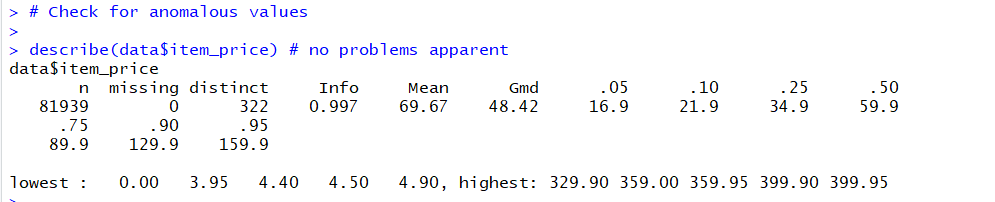
\includegraphics[width=0.95\linewidth]{4.describe_item_price}
	\caption{Describe Item Price}
	\label{fig:4}
\end{table}
\\
When putting customer id's and their order records together, we assign the new variable that we have created ''total.order.'' For this element, we think it also best suits as an indicator of frequency, as in how often a user does his or her shopping on this website. Therefore we rename it as ''Freq.'' Besides, we decide that it would be much more convenient to change the format in integer. \\
\subsubsection{Creating Recency of Last Order Variable}
Based on ''order date,'' we can get the recency of last order from the original data. We start off using .describe function to check if there is any anomalous value.\\
\begin{table}[h]
	\centering
	\includegraphics[width=0.95\linewidth]{"5.describe order date"}
	\caption{Decribe Order Date}
	\label{fig:5}
\end{table}\\
But since in this new project, we are no longer interested in how each order behaves, but rather, how each customer behaves. Hence, the ''order data'' in the original data set is not of much use to our project. The sole thing we need to know is when a user last ordered from the website. In other words, we need a new recency variable that could describe the last order of each customer, which will explain why we continue to name a new variable ''recency in months'' even though there could be some confusion in there when it seems there are two variables that both point to recency. But just keep in mind that the first one comes from the original data set and has not been transformed by any way. It refers to when each item was last ordered, though by whom we do not know. On the other hand, the second recency variable named ''recency.in.months'' that we created refers to when each customer last placed their order, as for what they have purchased is off the topic.

To create ''recency.in.month'', we use a similar approach that we have tried before with loyalty variable. First, we standardize the format of all order dates, then use \textbf{\textit{ceiling\_date function}} for arithmetic with dates, and save them all as numeric in the end. We aggregate all the order dates by the ''user\_id'' list to make them user oriented. Having created the new variable ''recency.in.months,'' we can omit all the irrelevant variables for this part, i.e. recency, item price, order item id, and order date.

\subsubsection{Putting Everyting Together}
To put everything together, we first change the column names from ''user\_id'' to ''ID'', for reasons of simplicity and convenience. In the meanwhile, we want to get rid of all the duplicates in the data set with the help of \textbf{\textit{.unique}} function. Using the \textbf{\textit{.sort}} function and setting ''decrease = true'' sort the ID vectors from largest to smallest. To merge the customer ID data frame to the original data set, we also need \textbf{\textit{.merge}} function to join these two data frames.

With the \textbf{\textit{.rm}} function, we remove all the irrelevant variables, i.e. total.value, total.orders and recency from the data set once and for all.

\subsubsection{Creation of RFM} 
The considered time period for the rfm is one year, i.e. 12 months. Hence, dividing the total orders by 12 gives ''frequency.per.month'', which means the variable ''total orders'' can be dropped. Meanwhile, dividing the total value by 12 gives us "monetary.per.month" and further the variable ''total value'' can be dropped. With\textbf{\textit{.cut}} function, we can get the counts of overall numbers into 10 groups of similar size. The scale is then the same for the three variables. If we give recency, frequency and monetary each a weight of 1/3 and calculate an average, we have our final for the RFM ranging from 0 to 10. \\
As explained in chapter 2, rfm is an important factor that reflects customer value and consists of three big questions.\\
\begin{figure}[h]
	\centering
	\includegraphics[width=0.95\linewidth]{"6.create rfm"}
	\caption{Create RFM}
	\label{fig:6}
\end{figure}\\
It is important to keep things simple while coding, so that it would not become too messy in the end. Therefore, having created rfm, the rest variables that we relied on such as ''recency.rfm,'' ''frequency.rfm,'' ''monetary.rfm,'' ''frequency.per.month,'' ''recency.in.month'' and ''monetary.per.month'' all become irrelevant. We will drop them all.

\subsubsection{Last Minor Changes}
Finally, the last step is to give the column a new name ''state'' and reorganize the columns of the data set in the order of, "ID", "state", "gender", "age", "loyalty.in.month" and "-rfm". We also want to make sure all variables are factorized, especially "gender" and "state".

In case there is any missing values in the final data set, we use \textbf{\textit{.complete.cases}} and pick them out to remove them. To make sure everyone will get the same result when running the same piece of code, we use \textbf{\textit{set.seed}} function to fix the seed to 1. This allows reproducibility of results when drawing samples. Considering the relatively large data set we indeed draw a sample from the original data set. Otherwise the complex calculations like the gower matrix would take too much time.


\subsection{Clustering Techniques}
\textbf{Motivation}: After the preliminary manipulation of existent data, we are ready for the next step: conducting cluster analysis. The aim is to construct groups with homogeneous properties out of large heterogeneous samples. We want for each group or cluster, to be as homogeneous as it can be, but in the meanwhile, as different as possible from one another.

\subsubsection{Distance/Dissimilarity Matrix}
The preprocessing process has succeeded in rearranging our data structure to a sample of 6 variables with 28178 observations. So far it is still a big mix of factor and numeric variables and thus hardly satisfactory to serve as the base of clustering analysis. Any clustering analysis textbook will start with a dissimilarity/distance matrix. We want to do exactly the same.

To compute all the pairwise dissimilarities (distances) between observations in the data set which is of mixed types of variables, we use \textbf{\textit{.daisy}} function as a starting point to calculate the dissimilarity matrix. By setting \textit{metric = ''gower,''} a generalization of Gower's formula is used. A quick summary gives the overlook of all statistics:\\
\begin{table}[h]
	\centering
	\includegraphics[width=0.95\linewidth]{"7.gower dist"}
	\caption{Gower Dist}
	\label{fig:7}
\end{table}\\
We continue to save it as matrix by using \textbf{\textit{.as.matrix,}} just to be sure. Then we use \textbf{\textit{.sample}} function as a test run to see what the most similar pair of data and most dissimilar pair of data are in this data set. This is not difficult to do as long as we identify the maximum as well as the minimum values in the dissimilarity matrix. The results are shown below, respectively.

\begin{figure}[h]
	\centering
	\includegraphics[width=0.95\linewidth]{"8.distance matrix 1"}
	\caption{Distance Matrix 1}
	\label{fig:8}
\end{figure}

As can be seen, two female customers form Bavaria share the most similar pattern. They are both in late 30's, and have a loyalty duration of 12 months on this website. Moreover, the rfm values for each of them that R has calculated for us indicate that they have exactly the same value.\\
\begin{figure}[h]
	\centering
	\includegraphics[width=0.7\linewidth]{"9.distance matrix 2"}
	\caption{Distance Matrix 2}
	\label{fig:9}
\end{figure}\\
On the other hand, a female customer from North Rhine-Westphalia and a male customer from Mecklenburg-Western Pomerania certainly are the most dissimilar pair in this sample. They are 59 and 24 years old respectively. One has been on the website for more than 2 years, while the other has been barely over half a year. The rfm values have shown big differences, too.

\subsubsection{Determining number of clusters }
The next step is to determine the number of clusters. Here we utilize silhouette width and silhouette plot to help us find it out. Silhouette provides a succinct graphical representation of how well each object lies within its cluster (Peter J. Rousseeuw (1987)). The silhouette ranges from -1 to +1, where a high value indicates that the object is well matched to its own cluster and poorly matched to neighboring clusters.


A \textbf{\textit{.for loop}} is used to simulate the number of clusters. Within the loop, for each i from 2 to 11, we use the \textbf{\textit{.pam}} function to partition the data into i clusters until all 10 loops run out and in the end we have 10 silhouette widths that come from the total mean of the individual silhouette width. \\
The code reads:
\begin{figure}[h]
	\centering
	\includegraphics[width=0.6\linewidth]{"10.loop for number of clusters"}
	\caption{Loop for Number of Clusters}
	\label{fig:10}
\end{figure}\\
The silhouette plot shows that the optimal number of clusters in our sample is 8.\\
\begin{figure}[h]
	\centering
	\includegraphics[width=0.53\linewidth]{"11.plot for number of clusters"}
	\caption{Plot for Number of Clusters}
	\label{fig:11}
\end{figure}\\

\subsubsection{Partitioning Clustering}%3.3.3
\textbf{3.3.3.1 PAM-Algotithm}
As the previous part has shown that 8 is the appropriate number for clusters, since silhouette width declines right after. We set k = 8 as the number of clusters in \textbf{\textit{.pam}} function and group the whole sample by clusters. The \textbf{\textit{.summary}} gives the partitioning results for 8 clusters. Take cluster 1 and 2 for example,\\
\begin{table}[h]
	\centering
	\includegraphics[width=0.95\linewidth]{"12.pam results summary 1"}
	\includegraphics[width=0.95\linewidth]{"12.pam results summary2"}
	\caption{PAM Results Summaries}
	\label{fig:12}
\end{table}\\

What's more, we also want to check medoids, namely, the most representative individual of each cluster.
\begin{table}[htp]
	\centering
	\includegraphics[width=0.95\linewidth]{"13.pam medoids"}
	\caption{PAM Medoids}
	\label{fig:13}
\end{table}\\
The t-SNE cluster visualization is shown as below. 
\begin{figure}[htp]
	\centering
	\includegraphics[width=0.7\linewidth]{"14.partitioning clustering"}
	\caption{Partitioning Clustering}
	\label{fig:14}
\end{figure}\\
From the graph, customers with similar characteristics are almost clustered in the same group. The overall picture looks neat. It can be easily seen that there 8 quite focused clusters. However, there are still some outliers scattering in the middle part of this graph that have failed to come together.\\
\\
\newline
\newline
\textbf{3.3.3.2 K-modes Algorithm}\\
The second clustering technique that we perform is k-modes clustering. By setting the modes to 8, again, we can draw a scatterplot of the result.\\
\begin{figure}[h]
	\centering
	\includegraphics[width=0.75\linewidth]{"15.K-modes algorithm"}
	\caption{K-modes Algorithm}
	\label{fig:15}
\end{figure}\\
The patches of different colors represent the clusters. For the most part, the circles are clustered together, but there are still scatterings here and there. \\
\subsubsection{Hierarchical Clustering}
\textbf{3.3.4.1 Divisive Clustering}
For divisive hierarchical clustering analysis of the sample, we can use \textbf{\textit{.diana}} function in R which performs such procedure. By setting ''diss = TRUE'' as well as ''keep.diss = TRUE,'' we  can compute the clustering of the dissimilarity matrix. We further create a plot for diana object for better visualization effect.
\newline
In such a plot for diana object, the banner displays the hierarchy of clusters, and is therefore equivalent to a clustering tree. Heights represent bars between the observations. The divisive hierarchical clustering tree with our data set looks like this:\\
\begin{figure}[h]
	\centering
	\includegraphics[width=0.7\linewidth]{"17.Divisive clustering 2"}
	\caption{Divisive Clustering}
	\label{fig:17}
\end{figure}\\
At level about 0.6, we can cut the tree into 3 clusters. However, at level 0.58, we can cut the clustering tree into about 13 clusters. As discussed earlier, it is quite subjective to have an agreed-upon number of clusters to cut the clustering tree in hierarchical clustering analysis. The final conclusion, if there is one to speak of, largely depends on how the tree is cut and particularly at what level it is cut.\\
\\
\textbf{3.3.4.2 Agglomerative Clustering}\\
\\
Apart from divisive hierarchical clustering analysis, there is another way to do it. That is through agglomerative clustering, which uses \textbf{\textit{.hclust}} function in R. Here we decide to adopt \textit{the complete linkage} method to find compact, spherical clusters. After applying \textbf{\textit{.hclust}} function, we again use \textbf{\textit{.plot}} function to get a visualized clustering tree.\\
\begin{figure}[h]
	\centering
	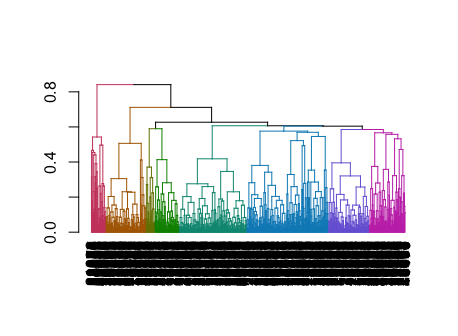
\includegraphics[width=0.7\linewidth]{18.agglomerative}
	\caption{Agglomerative}
	\label{fig:18}
\end{figure}\\
It can be seen that at level 0.6, we can cut the clustering tree into 4 clusters. However, if we cut it at level 0.58, there are 6 clusters. The result does not coincide with that of divisive clustering analysis. But we cannot reject either for sure, since the graph is hard to read and even with the tiniest error, the result could turn out to be drastically different.\\

\subsubsection{Density-Based Clustering-DBSCAN Algorithm}
\textbf{Motivation}  Besides the two essential clustering methods: hierarchical algorithms and partitioning methods, we are also interested in clustering methods based on density, which involves the implementation and use of the R package \textbf{\textit{dbscan}}, given its unique features and advantages.

To apply DBSCAN, we need to decide on the neighborhood radius \textbf{\textit{eps}} and the density threshold \textbf{\textit{minPts}}. For \textbf{\textit{minPts}}, the rule of thumb is to use the number of dimensions of the data set plus one. In our case, we set it to 5. For \textbf{\textit{eps}}, we call for \textbf{\textit{.plot}} function to plot the density as well as empirical cumulative density function for the dissimilarity matrix.
\begin{figure}[h!]
	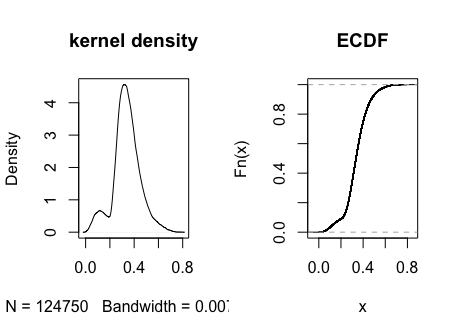
\includegraphics[width=0.7\linewidth]{19.DBSCAN}
	\caption{DBSCAN}
	\label{fig:19}
\end{figure}\\
And then we install and implement the dbscan package and call .dbscan function to give it a quick run of the complete the density-based clustering analysis. \\

\newpage
\section{Evaluation of different techniques }		
In our report we analyze 3 groups of clustering techniques. In order to compare these techniques we will provide with analysis of each algorithm based on available literature.

First group is partitioning clustering where we compute PAM-algorithm and K-modes algorithm. Partitioning algorithms are clustering techniques that subdivide the data sets into a set of k groups, where k is the number of groups pre-specified by the analyst. There are different types of partitioning clustering methods. The most popular is the K-means clustering MacQueen (1967), in which, each cluster is represented by the center or means of the data points belonging to the cluster. The K-means method is sensitive to outliers. However we used an alternative to k-means clustering is the K-medoids clustering or PAM (Partitioning Around Medoids, Kaufman and Rousseeuw (1990)), which is less sensitive to outliers compared to k-means.

Furthermore, the standard k-means algorithm isn't directly applicable to categorical data, for various reasons. The sample space for categorical data is discrete, and doesn't have a natural origin. A Euclidean distance function on such a space isn't really meaningful. In order to compute K-means algorithm we need translating our data into vectors what was difficult and time expensive. But, instead of this we used an algorithm called K-modes that works directly on this type of data. The advantages and disadvantages of partitioning clustering methods Sisodia et al. (2012) are:

\textbf{Advantages}
\begin{itemize}
	\item Relatively scalable and simple,
	\item Suitable for datasets with compact spherical clusters that are well-separated.
\end{itemize}
\textbf{Disadvantages}
\begin{itemize}
	\item Severe effectiveness degradation in high dimensional spaces as almost all pairs of points are about as far away as average; the concept of distance between points in high dimensional spaces is ill-defined,
	\item Poor cluster descriptors,
	\item Reliance on the user to specify the number of clusters in advance,
	\item High sensitivity to initialization phase, noise and outliers,
	\item Frequent entrapments into local optima,
	\item Inability to deal with non-convex clusters of varying size and density.
	
\end{itemize}
Second group was hierarchical clustering, and we implemented divisive clustering and agglomerative clustering. Hierarchical clustering is an alternative approach to partitioning clustering for identifying groups in the dataset. It does not require to prespecify the number of clusters to be generated. The result of hierarchical clustering is a tree-based representation of the objects, which is also known as dendrogram, like the one shown in Figure 4.1. Observations can be subdivided into groups by cutting the dendrogram at a desired similarity level.\\
\begin{figure}[h!]
	\centering
	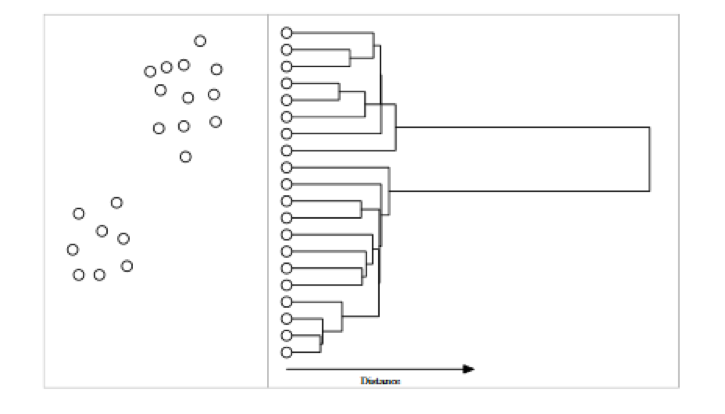
\includegraphics[width=0.7\linewidth]{21.Dendrogram}
	\caption{Theoretical Dendrogram}
	\label{fig:21}
\end{figure}\\
Agglomerative clustering: It's also known as AGNES (Agglomerative Nesting). It works in a bottom-up manner. That is, each object is initially considered as a single-element cluster (leaf). At each step of the algorithm, the two clusters that are the most similar are combined into a new bigger cluster (nodes). This procedure is iterated until all points are member of just one single big cluster (root). The result is a tree which can be also plotted as a dendrogram (Figure 4.1).

Divisive hierarchical clustering: It's also known as DIANA (Divise Analysis) and it works in a top-down manner. The algorithm is an inverse order of AGNES. It begins with the root, in which all objects are included in a single cluster. At each step of iteration, the most heterogeneous cluster is divided into two. The process is iterated until all objects are in their own cluster (Figure 4.1).

\begin{figure}[h]
	\centering
	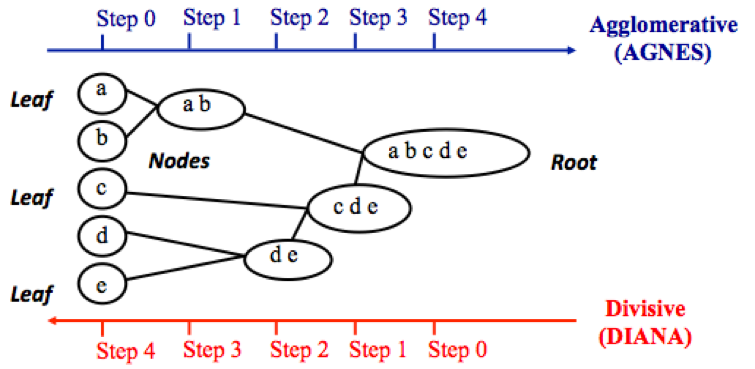
\includegraphics[width=0.7\linewidth]{20.Agnes_Diana_Algorithms}
	\caption{AGNES vs. DIANA}
	\label{fig:20}
\end{figure}
According to the work of Sonagara and Badheka (2014), following advantages and disadvantages of hierarchical clustering can be distinguished. 
\textbf{Advantages}
\begin{itemize}
	\item Embedded flexibility concerning the extent of granularity,
	\item Ease of handling of any types of similarity or distance,
	\item Consequently, the applicability to any attribute varieties.
\end{itemize}
\textbf{Disadvantages}
\begin{itemize}
	\item Vagueness of termination criteria,
	\item The undeniable fact that most hierarchical algorithms don't revisit.	
\end{itemize}
It worth noticing that based on set of literature on this topic, we can conclude that divisive clustering is good at identifying large clusters while agglomerative clustering is good at identifying small clusters.

It is clear that a distinction among different types of clusterings is whether the set of clusters is nested or unnested. Comparing partitioning and hierarchical clustering algorithms we can conclude that a partitional clustering is simply a division of the set of data objects into non-overlapping subsets (clusters) such that each data object is in exactly one subset meanwhile a hierarchical clustering is a set of nested clusters that are organized as a tree. Hierarchical clustering can be seen as a sequence of partitional clusterings and a partitional clustering can be obtained by cutting the hierarchical tree at a particular level.

Moreover, hierarchical clustering useful if the underlying application has taxonomy. But this type of clustering algorithms is expensive in terms of their computational and storage requirements. Besides that, merges are final and cannot be undone at a later time, preventing global optimization and causing trouble for noisy, high-dimensional data.The last group is Density based clustering (here we used DBSCAN algorithm). DBSCAN is a well-known algorithm for density-based clustering because it can identify the groups of arbitrary shapes and deal with noisy datasets. However, with the increasing amount of data, DBSCAN algorithm running on a single machine has to face the scalability problem. The main argument to use this technique is it shows good efficiency on large databases, i.e. on databases of significantly more than just a few thousands objects.

According to paper of Sharma et al. 2012 DBSCAN algorithm have following 
\textbf{advantages}:
\begin{itemize}
\item It does not require you to know the number of clusters in the data a priori, as opposed to k-means,
\item DBSCAN can find arbitrarily shaped clusters. It can even find clusters completely surrounded by (but not connected to) a different cluster. Due to the MinPts parameter, the so-called single-link effect (different clusters being connected by a thin line of points) is reduced,
\item DBSCAN has a notion of noise,
\item DBSCAN requires just two parameters and is mostly insensitive to the ordering of the points in the database. Only points sitting on the edge of two different clusters might swap cluster membership if the ordering of the points is changed, and the cluster assignment is unique only up to isomorphism.
\end{itemize} 
However, DBSCAN cannot cluster data sets well with large differences in densities.\\
Other \textbf{disadvantages} of DBSCAN Sisodia et. al. (2012):\\
\begin{itemize}
	\item High sensitivity to the setting of input parameters,
	\item Poor cluster descriptors,
	\item Unsuitable for high-dimensional datasets because of the curse of dimensionality phenomenon. 
\end{itemize}
Based on different sources of literature we can conclude that all these group of clustering techniques has wide applications in pattern recognition, spatial data analysis, image processing, economic science (especially market research).\\

\section{Conclusion}
In this report, we analyzed the real-world data of an online retailer to investigate the clustering of consumers purchasing preferences from their purchasing record and analyze efficiency of different clustering techniques. We applied the programming language R throughout the work and created two quantlets. 

As first steps, we analyzed theoretical aspects of cluster analysis in the context of mixed type data. There we distinguish types of clustering methods and analyze the main features and principles of each group and technique based on current literature.

At the second stage, we preprocessed the data ridding irrelevant variables and creating new useful variables based on given information. According business logic, the crucial step for better understanding of customer features our work was creating RFM variable to represent customer value. We can conclude that for the analysis of an online retail data, it is necessary to compute analytical procedure and rearrange data set by dropping useless information, removing outliers, normalizing missing data and creating new variables based on business logic.

After preprocessing the date, in order to construct groups with homogenous properties out of large heterogeneous samples, we implemented following groups of clustering techniques: partitioning clustering, hierarchical clustering, density based clustering.

In the last section we made analysis of current literature in order to compare different techniques and algorithms. Thus, group of partitioning clustering techniques include the simplest algorithms as compared to other algorithm. Meanwhile, density based clustering is the most complicated technique which that has been used. To sum it up, most of the clustering techniques (excluding of DBSCAN algorithm) perform bad on large databases. However, each method has its advantages and disadvantages and performance depends on features of dataset. There is not universal technique which will suit every type of data.


\newpage

\section*{Bibliography}
Birant, D. and Kut, A. (2007). \textit{ST-DBSCAN: An algorithm for clustering spatial?temporal data.} Data \& Knowledge Engineering, 60(1), pp.208-221.\\
\textbf{URL:} \url{http://www.sciencedirect.com/science/article/pii/S0169023X06000218}\\
\\
Han J. and Kamber M. Data Mining: \textit{Concepts and Techniques}, The Morgan Kaufmann Series in Data Management Systems, ISBN:  978-0-12-381479-1, San Francisco, 2000. \\
\textbf{URL:} \url{https://www.elsevier.com/books/data-mining-concepts-and-techniques/han/978-0-12-381479-1}\\
\\
Härdle, W. and L. Simar (2003): \textit{Applied Multivariate Statistical Analysis.} Springer, New York.\\
\\
Meert, W., \textit{Clustering Maps}, Thesis submitted for the program Master of Artificial Intelligence, academic year 2005-2006\\
\textbf{URL:} \url{https://pdfs.semanticscholar.org/09d6/39042005b92597 c5c6bcf47b19e7bfc8ee3d.pdf}\\
\\
Morissette, L., Chartier, S. (2013). \textit{The k-means clustering technique : General considerations and implementation in Mathematica}. \\
\textbf{URL:} \url{https://pdfs.semanticscholar.org/c7d8/639b2b087ada8218f4e241fc9750f3691645.pdf?_ga=2.175648417.2062796574.1533981083-1241178131.1533981083}\\
\\
Reynolds, A., Richards, G., de la Iglesia, B. and Rayward-Smith, V. (2006). \textit{Clustering Rules: A Comparison of Partitioning and Hierarchical Clustering Algorithms.} Journal of Mathematical Modelling and Algorithms, 5(4), pp.475-504.\\
\textbf{URL:} \url{http://dblp.uni-trier.de/db/journals/jmma/jmma5.html#ReynoldsRIR06}\\
\\
Rousseeuw, Peter J. (1987). \textit{Silhouettes: a Graphical Aid to the Interpretation and Validation of Cluster Analysis.} Computational and Applied Mathematics. 20: 53-65. \\
\textbf{URL:} \url{http://www.sciencedirect.com/science/article/pii/0377042787901257}\\
\\
Sharma, N., Bajpai, A. and Litoriya, R. (2012). \textit{Comparison the various clustering algorithms of weka tools. International Journal of Emerging Technology and Advanced Engineering}, 2(5).\\ \textbf{URL:} \url{http://www.ijetae.com}\\
\\
Shrivastava, V., Arya, P.N. (2012). \textit{A Study of Various Clustering Algorithms on Retail Sales Data.}, \\
\textbf{URL:} \url{https://pdfs.semanticscholar.org/9a6b/470963636a7f9499492ab9a3f0ad99dd5ae2.pdf}
\\
Simovici, Dan A.(2011)\textit{The PAM Clustering Algorithm}, CS738, Data Mining, University of Massachusetts Boston\\
\textbf{URL:} \url{https://www.cs.umb.edu/cs738/pam1.pdf}\\
\\
Sisodia, D., Singh, L., Sisodia, S. and Saxena, K. (2012). \textit{Clustering Techniques: A Brief Survey of Different Clustering Algorithms.} International Journal of Latest Trends in Engineering and Technology, 1(3).\\
\textbf{URL:} \url{https://pdfs.semanticscholar.org/68d8/a39bc9035fef6ec504cbd04e900cadd504aa.pdf}\\
\\
Sonagara, D. and Badheka, S. (2014). \textit{Comparison of Basic Clustering Algorithms.} Monthly Journal of Computer Science and Information Technology, 3(10), pp.58-61.\\
\textbf{URL:} \url{https://pdfs.semanticscholar.org/f0a4/d6bfb37b6c1102f7ef6b0d0f2ef861da6aca.pdf}\\






















\end{document}
